\documentclass{article}

\usepackage[final]{neurips_2022}
\usepackage[utf8]{inputenc} % allow utf-8 input
\usepackage[T1]{fontenc}    % use 8-bit T1 fonts
\usepackage{hyperref}       % hyperlinks
\usepackage{url}            % simple URL typesetting
\usepackage{booktabs}       % professional-quality tables
\usepackage{amsfonts}       % blackboard math symbols
\usepackage{nicefrac}       % compact symbols for 1/2, etc.
\usepackage{microtype}      % microtypography
\usepackage{xcolor}         % colors
\usepackage{amsmath}        % math symbols
\usepackage{authblk}        % for the author command
\usepackage{graphicx}

\title{
    Proofs for Excess Risk and Bias-Variance Tradeoff Values in Linear Regression: A Review of 
    Preetum Nakkiran's "More Data Can Hurt for Linear Regression: Sample-wise Double Descent"
}
\author{%
    \textbf{Shawn Santhoshgeorge} \quad \textbf{Anaqi As Shafiq Bin Amir Razif} \\
    University of Toronto Scarborough - STAD80 \\
    \texttt{\{shawn.santhoshgeorge,anaqi.amirrazif\}@mail.utoronto.ca}
}

\begin{document}

\maketitle

\begin{abstract}
    In overparameterized linear regression, the phenomenon of double descent can be observed in which the test mean squared error initially decreases with a fixed parameter $d$ and an increasing sample $n$. It keeps on decreasing before increasing asymptotically towards infinity when $n \approx d$ before it begins decreasing again. We call the regime where $n<d$ to be the overparameterized regime and the underparameterized regime is when $n > d$. There are interesting concepts that can be found when researching and analyzing these regimes especially around the area of $n \approx d$. One research that has been done for double descent for linear regression is the paper [Nakkiran, 2019] in which concepts such as the bias-variance tradeoffs in these regions are looked at. This review serves as a supplement to the [Nakkiran, 2019] paper as this review aims to provide proofs for some of the claims that were made in the [Nakkiran, 2019]. Specifically, a deeper analysis on Section 3.1 of [Nakkiran, 2019] will be conducted in this review.
\end{abstract}
\section{Introduction}

In the field of machine learning, the concept of the bias-variance tradeoff is well known in which the two are inversely related such that as one increases, the other tend to do the opposite. The task for researchers and data scientists is often to try and find the best balance between the two such that their values would yield the minimum test risk. It is the case such that if the model has more features d than it has samples n, then the model would overfit the training data where it fits not only the data but the noise that comes with it; leading to poor generalization in the testing phase.

In [Nakkiran, 2019] however, it is shown that this is not necessarily the case. In current machine learning research, the "double descent" phenomenon shows that even if the model is overparameterized where d>n and overfits the data, the model tends to generalize quite well in the testing phase. So both the underparameterized (n>d) and overparameterized (n<d) regimes yield low - or at least non-increasing - test risks as the number of features increase in comparison to the number of samples. The only intriguing case occurs when n $\approx$ d in which the test risk increases asymptotically towards infinity. 

The study [Nakkiran, 2019] analyzes this phenomenon and went in depth to find the different values of the bias and variance in each of the 3 regimes (overparameterization, underparameterization, n $\approx$ d). This review will supplement [Nakkiran, 2019] by providing and verifying the claims made in Section 3.1 of [Nakkiran, 2019] through proofs and examples.

\section{Problem Statement}
\subsection{Setup}

This review will use the exact problem setup that was implemented in [Nakkiran, 2019]. So, let the ground truth distribution D be $(x,y) \in \mathbb{R}^d \times \mathbb{R}$ where the covariates $x \sim N(0, I_d)$ and the response $y = <x, \beta> + \epsilon$ where $\beta$ is some unknown, arbitrary value such that $\|\beta\|_2 < 1$ and $\epsilon$ is the noise in the model such that $\epsilon \sim N(0, \sigma^2)$. Given are $n$ samples $(x_i,y_i)$ from D and the linear model is $f_{\hat{\beta}} = <x,\hat{\beta}>$. We want to learn this linear model by estimating $y$ given $x$. In other words, we want to find the estimator $\hat{\beta}$ such that it minimizes the test mean squared error (MSE):

\begin{align}
    R(\hat{\beta}) :&= \mathbb{E}_{(x,y)\sim D} [(<x,\hat{\beta}> - y)^2]\\
    &= \|\beta - \hat{\beta}\|^2 + \sigma^2
\end{align}

Lets perform this task using ridgeless linear regression with gradient descent that is initialized at 0. Thus, the empirical risk is:

\begin{align}
    min_{\hat{\beta}} \|X\hat{\beta} - y\|^2
\end{align}

where $X \in \mathbb{R}^{nxd}$ is the data matrix, $y \in \mathbb{R}^n$ is the response, and $\hat{\beta}$ is the estimator that we are trying to solve.

\subsection{Observations}

The solution found through the specified gradient descent at covergence as stated in [Nakkiran, 2019] is $\hat{\beta} = X^{\dagger}y$ where $\dagger$ denotes the Moore-Penrose inverse (i.e., $X^{\dagger} = (X^{T}X)^{-1}X^{T}$).

Furthermore, with a fixed d = 1000, the varying number of n samples will produce a non-monotonic test MSE graph in which the test MSE decreases in both the overparameterized regime ($n < d$) and the underparameterized regime (n>d) but goes up asymptotically towards infinity as stated when $n \approx d$.

$\textbf{Observation 1}$: In the underparameterized regime ($n > d$), the test MSE is monotone decreasing as the number of samples n increase. A simple explanation for this would be The Law of Large Numbers which states that the estimator of the mean of the data will converge to the ground truth mean as $n \rightarrow \infty$. A deeper proof can be seen rigorously in [Hastie et al., 2019].

$\textbf{Observation 2}$: In the overparameterized regime ($n < d$), there is an initial descent where the test MSE decreases as the number of samples increases. The reason for this is because the bias decreases with the increasing number of samples.

$\textbf{Observation 3}$: In the overparameterized regime but close to where $n \approx d$, we can observe the ascent behaviour in the graph in which the test MSE increases and peaks when $n=d$. This is due to the variance increasing and diverging at $n=d$.

As we can see, Observation 1 is intuitively explainable as classical regression models have underparameterized regimes. Observations 2 and 3 however, are less intuitive as though they demonstrate the bias-variance tradeoff, their overparametrized nature alongside the wrinkle when $n \approx d$ make them quite intriguing. These phenomenons will be focused on in this review just like how its mechanisms and intuitions were analyzed in [Nakkiran, 2019]. Specifically, this review will go into deeper investigation of Section 3.1 in [Nakkiran, 2019].



\subsection{Problem: Excess Risk and Bias-Variance Tradeoffs}

[Nakkiran, 2019] is concerned with investigating the bias-variance tradeoffs of all three observations specified above. This is found in Section 3.1 of the paper [Nakkiran, 2019]. This review will focus on further explaining how to achieve these results and not focus on any other parts of [Nakkiran, 2019] (i.e., Section 3.2, 3.3).

Formally, this review acknowledges that the solution $\hat{\beta} = X^{\dagger}y$ has multiple forms depending on which regime is being investigated. As stated in [Nakkiran, 2019]:

\begin{equation*}
\hat{\beta} = X^{\dagger}y =\begin{cases}
          argmin_{\beta : X\beta = y} \|\beta\|^2 \quad when \hspace{1mm} n\leq d \hspace{1mm} \textbf{("Overparameterized")}\\
          argmin_{\beta} \|X\beta\ - y\|^2 \quad when \hspace{1mm} n>d \hspace{1mm} \textbf{("Underparameterized")}
     \end{cases}
\end{equation*}

This review will analyze the bias and variance values for each of these cases in more depth than what was provided in Section 3.1 of [Nakkiran, 2019].

This review believes that it is important to explain how [Nakkiran, 2019] obtained these biases and variances in detail as [Nakkiran, 2019] stated its claim with minimal explanation and analysis. More specifically, this review believes that the rigorous proofs and examples of the excess risk and bias-variance tradeoffs analyses will help the reader have a deeper understanding of the concept at hand when it comes to the double descent phenomenon in sample-wise linear regression.

\section{Main Result}

This section will briefly mention the main results that came out of the bias and variance tradeoffs section in [Nakkiran, 2019]. Proofs of these results will be covered in Section 4 of this review.

[Nakkiran, 2019] shows that for the ground-truth parameter $\beta$, the excess risk of the estimator is:

\begin{align}
    \bar{R}(\hat{\beta}) := \|\beta - \hat{\beta}\|^2
\end{align}

Similarly, the expected excess risk over samples $(X,y) \sim D$ is then:

\begin{align}
    \mathbb{E}_{X,y} [\bar{R} (\hat{\beta}_{X,y}] = \|\beta - \mathbb{E}[\hat{\beta}]\|^2 + \mathbb{E} [\|\hat{\beta} - \mathbb{E} [\hat{\beta}]\|^2]
\end{align}

where $\|\beta - \mathbb{E}[\hat{\beta}]\|^2$ is the bias $B_n$ and $\mathbb{E} [\|\hat{\beta} - \mathbb{E} [\hat{\beta}]\|^2]$ is the variance $V_n$ of the estimator over n samples.

Then, [Nakkiran, 2019] also showed the exact values for how the bias and variance can be wrriten for the specific estimator $\hat{\beta} = X^{\dagger}y$ in the overparameterized regime:

\begin{align}
    &B_n = \| \mathbb{E}_{X \sim D^n} [Proj_{X^{\perp}} (\beta)] \|^2\\
    &V_n = \mathbb{E}_X [\|Proj_{X} (\beta) - \mathbb{E}_X [Proj_X (\beta)]\|^2] + \sigma^2 \mathbb{E}_X [Tr((XX^T)^{-1})]
\end{align}

where $Proj_X$ is the orthogonal projector onto the rowspace of the data $X\in\mathbb{R}^{n \times d}$, and $Proj_{X^{\perp}}$ is the projector onto the orthogonal complement of the rowspace as specified by [Nakkiran, 2019].

The proofs of the values of the bias (Equation (6)) and variance (Equation (7)) and the specific conditions of the specific estimator $\hat{\beta} = X^{\dagger}y$ can be found in the appendix of [Nakkiran, 2019].

These are $\textbf{not}$ the bias and variance that this review will focus on in terms of proofs as it has been done in [Nakkiran, 2019].



Instead, we will focus on the following claims:

\textbf{Claim 1}: This claim concerns itself with the overparameterized regime (n<d) and it first defines $\gamma := \frac{n}{d} < 1$ and then the bias and variance are:

\begin{align}
    &B_n = (1-\gamma)^2 \|\beta\|^2\\
    &V_n \approx \gamma (1-\gamma) \|\beta\|^2 + \sigma^2 \frac{\gamma}{1-\gamma}
\end{align}

This implies the expected excess risk for $\gamma < 1$ to be:

\begin{align}
    \mathbb{E} [\bar{R}(\hat{\beta}] \approx (1-\gamma)\|\beta\|^2 + \sigma^2 \frac{\gamma}{1-\gamma}
\end{align}

\textbf{Claim 2}: This claim concerns itself with the underparameterized regime (n>d) and it defines $\gamma := \frac{n}{d} > 1$ and then the bias and variance are:

\begin{align}
    &B_n = 0\\
    &V_n \approx \frac{\sigma^2}{\gamma - 1}
\end{align}



\section{Proofs and Examples}

In this section, we will prove the claims that are mentioned above as presented in [Nakkiran, 2019]. By that, we mean that we will show the proofs for equations (8), (9), (10), (11), and (12).

\subsection{Proof of Equation 8}

In [Nakkiran, 2019], it is stated that $Proj_X (\beta)$ is the projector onto a uniformly distributed $\emph{n}$-dimensional subspace. This fact is then said to imply that

\begin{align}
    \mathbb{E}[Proj_X (\beta)] = \gamma \beta
\end{align}

which then implies 

\begin{align}
    \mathbb{E} [\|Proj_X (\beta)\|^2] = \gamma \|\beta\|^2
\end{align}

To prove Equation (8) (and Equation (9)), we must first prove Equations (13) (and (14)).

\subsubsection{Proof of Equation 13}

\emph{Proof.}
Let $Proj_X (\beta)$ be the orthogonal projector onto the rowspace of the data $X\in \mathbb{R}^{n \times d}$.

\underline{WTS}: $\mathbb{E} [Proj_X (\beta)] = \gamma \beta$

We refer the reader to Lemma 5.3.2 of [Vershynin, 2018] for the details of this proof. Furthermore, the reader can find this expression applied in [Ribeiro, 2023] for further studies. We believe that since the proof is already rigorous, it would be redundant for us to restate here in this review. 

\subsubsection{Proof of Equation 14}

\emph{Proof.}
Again, let $Proj_X (\beta)$ be the orthogonal projector onto the rowspace of the data $X\in \mathbb{R}^{n \times d}$. We can use the results from Equation (13) to help us prove Equation (14).

\underline{WTS}: $\mathbb{E} [\|Proj_X (\beta)\|^2] = \gamma \|\beta\|^2$ 

\begin{align*}
    \mathbb{E} [\|Proj_X (\beta)\|^2] &= \mathbb{E} [\|X^{T}(XX^{T})^{-1}X\beta\|^2]\\
    &= \mathbb{E} [X^{T}(XX^{T})^{-1}XX^{T}(XX^{T})^{-1}X\|\beta\|^2]\\
    &= \mathbb{E} [X^{T}(XX^{T})^{-1}X\|\beta\|^2]\\
    &= \mathbb{E} [Proj_X (\|\beta\|^2)]\\
    &= \gamma \|\beta\|^2
\end{align*}

as wanted.



\subsubsection{Proof of Equation 8 using Equations 13 (and 14)}

Now that we have proved Equations (13) and (14), we can move on to prove Equation (8). 

\emph{Proof.}
Let the setup be the same as the ones in Section 4.1.1 and 4.1.2. \\
Also, let $B_n = \|\mathbb{E} [Proj_{X^\perp} (\beta)]\|^2$ as seen in Equation (6) with the appropriate setup as well. This is because [Nakkiran, 2019] has stated this value for the bias in the overparameterized regime for the specific estimator $\hat{\beta} = X^{\dagger}y$ as mentioned in Section 3 of this review.

\underline{WTS}: $B_n = (1-\gamma)^2 \|\beta\|^2$

\begin{align*}
    B_n &= \|\mathbb{E}_{X \sim D^n}[Proj_{X^\perp} (\beta)]\|^2\\
    &= \|\beta - \mathbb{E}_{X \sim D^n} [Proj_X (\beta)]\|^2\\
    &= \|\beta - \gamma \beta\|^2\\
    &= \|(1-\gamma)\beta\|^2\\
    &= (1-\gamma)^2 \|\beta\|^2
\end{align*}

as wanted.

\subsection{Proof of Equation 9}

\emph{Proof.}
Similar to Section 4.1, let the setup for this proof be exactly the same. Furthermore, let $V_n =  \mathbb{E}_X [\|Proj_{X} (\beta) - \mathbb{E}_X [Proj_X (\beta)]\|^2] + \sigma^2 \mathbb{E}_X [Tr((XX^T)^{-1})]$ as seen in Equation (7).

\underline{WTS}: $V_n \approx \gamma(1-\gamma) \|\beta\|^2 + \sigma^2 \frac{\gamma}{1-\gamma}$

\begin{align*}
    V_n &= \mathbb{E}_X [\|Proj_{X} (\beta) - \mathbb{E}_X [Proj_X (\beta)]\|^2] + \sigma^2 \mathbb{E}_X [Tr((XX^T)^{-1})]\\
    &= \mathbb{E}_X [\|Proj_X (\beta)\|^2] - \mathbb{E}_X [\| \mathbb{E}_X [Proj_X (\beta)]\|^2] + \sigma^2 \mathbb{E}_X [Tr((XX^T)^{-1})]\\
    &= \gamma\|\beta\|^2 - \mathbb{E}_X [\|\gamma\beta\|^2] + \sigma^2 \mathbb{E}_X [Tr((XX^T)^{-1})]\\
    &= \gamma\|\beta\|^2 - \mathbb{E}_X [\gamma^2 \|\beta\|^2] + \sigma^2 \mathbb{E}_X [Tr((XX^T)^{-1})]\\
    &= \gamma\|\beta\|^2 - \gamma^2\|\beta\|^2 + \sigma^2 \mathbb{E}_X [Tr((XX^T)^{-1})]\\
    &= (\gamma - \gamma^2) \|\beta\|^2 + \sigma^2 \mathbb{E}_X [Tr((XX^T)^{-1})]\\
    &= \gamma(1-\gamma) \|\beta\|^2 + \sigma^2 \mathbb{E}_X [Tr((XX^T)^{-1})]\\
    &\approx \gamma(1-\gamma) \|\beta\|^2 + \sigma^2 \frac{\gamma}{1-\gamma}
\end{align*}

as wanted.

Note that $\mathbb{E}_X [Tr((XX^T)^{-1})]$ converges to $ \frac{\gamma}{1-\gamma}$ in large samples of $n$ and $d$ as stated in [Nakkiran, 2019]. Though this fact is first seen in [Marčenko and Pastur, 1967] and also used as an example in [Hastie et al., 2019]. We refer the reader to these papers to have a better understanding of the effect.



\subsection{Proof of Equation 10}

\emph{Proof.}
Here we assume the overparameterized setup that was seen in Section 4.1 and Section 4.2.

We have already defined: 
$B_n = (1-\gamma)^2 \|\beta\|^2$ and 
$V_n \approx \gamma (1-\gamma) \|\beta\|^2 + \sigma^2 \frac{\gamma}{1-\gamma}$

We also know that: $\mathbb{E}_{X,y} [\bar{R} (\hat{\beta}_{X,y}] = B_n + V_n$ in Equation (5)

\underline{WTS}: $\mathbb{E}_{X,y} [\bar{R} (\hat{\beta}_{X,y})] \approx (1 - \gamma) \|\beta\|^2 + \sigma^2 \frac{\gamma}{1-\gamma} = (1- \frac{n}{d}) \|\beta\|^2 + \sigma^2 \frac{n}{d-n}$

\begin{align*}
    \mathbb{E}_{X,y} [\bar{R} (\hat{\beta}_{X,y})] &= B_n + V_n\\
    &\approx (1-\gamma)^2 \|\beta\|^2 + \gamma (1-\gamma) \|\beta\|^2 + \sigma^2 \frac{\gamma}{1-\gamma}\\
    &= ((1-\gamma)^2 + \gamma(1-\gamma)) \|\beta\|^2 + \sigma^2 \frac{\gamma}{1-\gamma}\\
    &= (1-2\gamma+\gamma^2+\gamma-\gamma^2)\|\beta\|^2 + \sigma^2 \frac{\gamma}{1-\gamma}\\
    &= (1-\gamma) \|\beta\|^2 + \sigma^2 \frac{\gamma}{1-\gamma}\\
    &= (1-\frac{n}{d}) \|\beta\|^2 + \sigma^2 \frac{\frac{n}{d}}{1-\frac{n}{d}}\\
    &= (1-\frac{n}{d}) \|\beta\|^2 + \sigma^2 \frac{\frac{n}{d}}{\frac{d-n}{d}}\\
    &= (1-\frac{n}{d}) \|\beta\|^2 + \sigma^2 \frac{n}{d-n}
\end{align*}

as wanted.

\subsection{Proofs of Equation 11 and Equation 12}

Please refer to [Hastie, et al., 2019] for the completeness of these claims for the values of the bias and variance in the underparameterized regime. That being said, here is a simple version of the proof for the bias value in the underparameterized regime:

\emph{Proof of Equation 11.}
Let $\hat{\beta} = X^{\dagger}y = (X^{T}X)^{-1}X^{T}y$ in the underparaterized regime. Also, as defined in Section 2.1, $y = X\beta + \epsilon$.

\underline{WTS}: $B_n = 0$

\begin{align*}
    B_n &= \|\beta - \mathbb{E}[\hat{\beta}]\|^2\\
    &= \|\beta - \mathbb{E}[(X^{T}X)^{-1}X^{T}y]\|^2\\
    &= \|\beta -  \mathbb{E} [(X^{T}X)^{-1}X^{T} (X\beta + \epsilon)]\|^2\\
    &= \|\beta - \mathbb{E} [(X^{T}X)^{-1}(X^{T}X)\beta + (X^{T}X)^{-1}X^{T}\epsilon]\|^2\\
    &= \|\beta - \mathbb{E}[I\beta] + \mathbb{E} [(X^{T}X)^{-1}X^{T}\epsilon]\|^2\\
    &= \|\beta - \mathbb{E}[\beta] + 0]\|^2\\
    &= \|\beta - \beta\|^2\\
    &= \|0\|^2\\
    &= 0
\end{align*}

as wanted.

It is worth noting that $\mathbb{E} [(X^{T}X)^{-1}X^{T}\epsilon] = 0$ because $\epsilon \sim N(0, \sigma^2)$ so the expectation for $\epsilon$ is simply 0. This process can also be seen in Appendix A.1 of [Nakkiran, 2019].

\emph{Proof of Equation 12.}
For the proof of the value of the variance in an underparameterized regime, we refer the reader solely to [Hastie, et al., 2019] for a rigorous and complete proof as we believed it is redundant for us to restate the proof here.

\subsection{Excess Risk for the Underparameterized Regime}

An interesting observation that comes from the underparameterized regime is that the excess risk is exactly the same as the variance:

\begin{align*}
    \mathbb{E}_{X,y} [\bar{R} (\hat{\beta}_{X,y})] &= B_n + V_n\\
    &= 0 + V_n\\
    &\approx \frac{\sigma^2}{\gamma - 1}\\
\end{align*}

This makes sense not only because $B_n = 0$, but also because in the underparameterized regime, $n>d$ which means that as the number of samples $n$ increases, the risk only comes from the variance of the model. 



\section{Empirical Studies}

In this section, we wanted to confirm that these values are accurate empirically. Therefore, we created a linear regression using R with the exact setup as specified in Section 2.1 and plotted out the Test Risk against the increasing samples $n$. 

\begin{figure}[h!]
  \centering
  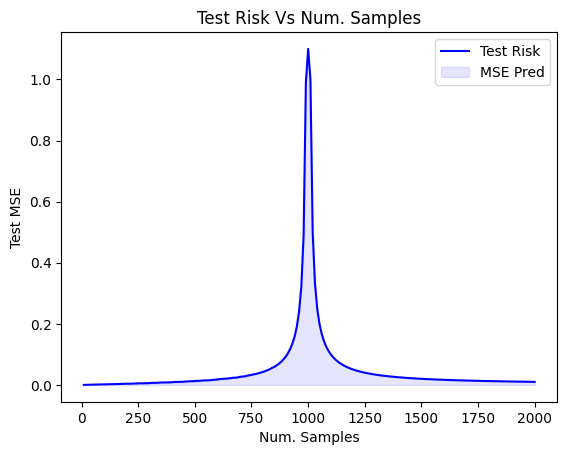
\includegraphics[width=0.75\textwidth, quiet]{graph.png}
\end{figure}

We found that we were able to recreate the plot that is found in Page 1 of [Nakkiran, 2019] which implies that the values that were proven theoretically in the previous section holds in an empirical setting as well.

The code for the plot above can be found \href{https://github.com/ShawnGeorge03/STAD80-Final-Paper/tree/main}{here} in our GitHub repository.

\underline{Note}: At $n=1000$, $\gamma = 1$ which means that there is a division by zero in the variance of the underparametrized regime as $V_n \approx \frac{\sigma^2}{\gamma - 1}$ in that regime (it would have faced the same problem if we ran the overparameterized model of the variance instead as well, we just chose to let the model use the underparameterized values for when $n=d$). So, to fix this issue, we decided to let $\gamma = n + \sigma = 1.1$ for whenever $n=d$. We believe that this choice for $\gamma$ is justified and the resulting model accurately reflects what we are trying to achieve in the first place.

\section{Limitations}

The limitations that exist in both this review and [Nakkiran, 2019] is that these processes and claims only apply to ridgeless linear regression. Furthermore, it is solely limited to the setup that has been defined in Section 2.1 with specifically an isotopic Gaussian distribution. This limitation means that the results in the [Nakkiran, 2019] paper cannot be used for other setups and machine learning models. So, even though the results might let us understand the "double descent" phenomenon in a slightly better light, the extension of these results can be quite limited in the machine learning field.

In [Nakkiran, 2019] specifically, some of the claims that were made in the paper lacks proper explanations such as the claims that were made regarding the bias and variance values. This limitation is exactly the reason this review was made, which was to explain how those values were achieved which was explain in Section 4 of this review.



\section{Future Directions}

The natural progression that comes from [Nakkiran, 2019] and this review is to address the limitations that have been discussed in Section 6. Therefore, further studies into other machine learning problems such as neural networks, decision forests, etc., regarding the double descent phenomenon should be conducted. Granted, there already exist some studies regarding the topic such as [Nakkiran et al., 2019, Hastie, 2019, Belkin, et al., 2018, Spigler et al., 2018, Geiger et al., 2019]. There also has been recent studies published this year that focuses itself on overparameterized linear regression as well such as [Ribeiro and Schön, 2023] that analyzed the effects of adversarial attacks on the model and [Wu and Xu, 2020] which discussed the optimal weighted $l_2$ regularization of the overparamterized linear regression model.

That being said, in a world that dives deeper and deeper into machine learning with overparameterized models in the age of big data, more research must be done to figure out the "double descent" phenomenon.

\section*{References}

[Belkin et al., 2018] Belkin, M., Hsu, D., Ma, S., and Mandal, S. (2018). Reconciling modern machine
learning and the bias-variance trade-off. arXiv preprint arXiv:1812.11118.

[Geiger et al., 2019] Geiger, M., Spigler, S., d’Ascoli, S., Sagun, L., Baity-Jesi, M., Biroli, G., and Wyart,
M. (2019). Jamming transition as a paradigm to understand the loss landscape of deep neural networks.
Physical Review E, 100(1):012115.

[Hastie et al., 2019] Hastie, T., Montanari, A., Rosset, S., and Tibshirani, R. J. (2019). Surprises in highdimensional ridgeless least squares interpolation. arXiv preprint arXiv:1903.08560.

[Marčenko and Pastur, 1967] Marčenko, V. A. and Pastur, L. A. (1967). Distribution of eigenvalues for some
sets of random matrices. Mathematics of the USSR-Sbornik, 1(4):457

[Nakkiran, 2019] Nakkiran, P. (2019). More Data Can Hurt for Linear Regression: Sample-wise Double Descent. arXiv preprint arXiv:1912.07242.

[Nakkiran et al., 2019] Nakkiran, P., Kaplun, G., Bansal, Y., Yang, T., Barak, B., and Sutskever, I. (2019).
Deep double descent: Where bigger models and more data hurt. arXiv preprint arXiv:1912.02292.

[Ribeiro and Schön] Ribeiro, A. H., Schön, Thomas B. (2023). Overparameterized Linear Regression under Adversarial Attacks. arXiv preprint arXiv:2204.06274.

[Spigler et al., 2018] Spigler, S., Geiger, M., d’Ascoli, S., Sagun, L., Biroli, G., and Wyart, M. (2018). A
jamming transition from under-to over-parametrization affects loss landscape and generalization. arXiv
preprint arXiv:1810.09665.

[Vershynin, 2018] Vershynin, R. (2018). High-Dimensional Probability, ser. Cambridge series in statistical and probabilistic mathematics. Cambridge University Press.

[Wu and Xu, 2020] Wu, D., Xu, J. (2020). On the Optimal Weighted `2 Regularization in Overparameterized Linear Regression. arXiv preprint arXiv:2006.05800.

\end{document}